\documentclass[12pt]{article}
\usepackage{lingmacros}
\usepackage{tree-dvips}
\usepackage[utf8x]{inputenc} % Включаем поддержку UTF8 
\usepackage[russian]{babel} 
\usepackage{mathtools}
\usepackage{graphicx}
\usepackage{amsmath}

\usepackage{skak}


\graphicspath{{pict/}}
\DeclareGraphicsExtensions{.pdf,.png,.jpg}

\DeclarePairedDelimiter{\ceil}{\lceil}{\rceil}

\begin{document}

\section*{Решения}

\subsection*{Задача 3.1}
Необходимо расставить ладьи одного цвета так, что на одной горизонтали с каждой из них было еще 3 и на одной вертикали 3 другие. Таким образом, в каждой строке или столбце ровно 4 ладьи одного цвета. Например:\\
\newgame
 
\fenboard{rrrr4/rrrr4/rrrr4/rrrr4/4RRRR/4RRRR/4RRRR/4RRRR w - - 0 20}
\showboard\\
Ответ: 16.

\subsection*{Задача 3.2}
Обе функции в левой и правой частях уравнения выпуклые, единственный корень у уравнения возникает тогда, когда $y = a^x$ касается прямой $y = x$, то есть $f(x_0) = x_0$ и $f'(x_0) = a^{x_0} \ln a = 1$. Отсюда $x_0 = \frac{1}{\ln a}$, т.е. $e = a^{\frac{1}{\ln a}} = \frac{1}{\ln a}$, $\ln a = \frac{1}{e}$, $a = e^{\frac{1}{e}} = 1.44466786$.
Ответ: 1.44466786.
\subsection*{Задача 3.3}
Количество слов из 3 букв длиной n $W_n = 3^N$. Так $W = 3^3 + 3^4 + 3^5 + 3^6 = 1080$.
Ответ: 1080.
\subsection*{Задача 3.4}
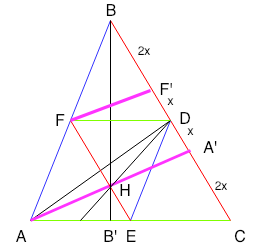
\includegraphics{math34}\\
Рассмотрим $\triangle ABC$: $DE, EF, DF$ -- медианы, $AA', BB'$ -- высоты. $BD = DC$. В $\triangle ADE$: медианы пересекаются в точке $H$, которая разделяет их в отношении $2:1$. Из подобия треугольников очевидно, что $DA':A'C = 1:2$. 
Пусть $AD = x$, $A'C = 2x$. $FH = 2 \cdot (HE + HE/2) - HE = 2HE = 2x$ По свойству паралелограмма, образованного медианами $FE$ и $BC$, перпендикулярами $AA'$ и $FF'$: $FH = F'A' = 2x$ и $FF'=HA'$, $F'D = x$. Также из подобия треугольников $BF' = 2x$, $FF'=HA'=AH$. \\
Рассмотрим $\triangle BA'H\sim\triangle AHE$(по 2 углам). $A'B:A'H=A'H:HE \Rightarrow A'H = \sqrt{A'B\cdot HE} = \sqrt{4x^2} = 2x = EF'=BF'$. 
Так, $\triangle BF'F$ -- прямоугольный равнобедренный, и угол при основании $\angle FBF' = 45^\circ$.\\
Ответ: 45.
\subsection*{Задача 3.5}
Все натуральные числа вида $(1 + x^n)$, где $n$ -- нечетное число, делятся нацело на $(1+x)$. \\
Таким образом, вычеркнем все числа, где $n$ = 1, 3, 5, 7, 9, 11 и 13. 15 оставляем.\\
Далее заменим $x^2$ на $y$. По аналогии вычеркнем числа, где n = 2, 6, 10. 14 оставляем.\\
Далее заменим $x^3$ на $z$. $n$ = 3, 9 -- вычеркнуты. 15 оставляем. 
Далее заменим $x^4$ на $w$. По аналогии вычеркнем число, где $n$ = 4. 12 оставляем.\\
Далее заменим $x^5$ на $v$. $n$ = 5 вычеркнуто. 15 оставляем. \\
Далее нет смысла перебирать, так как $3n > 15$. Оставшиеся числа взаимнопростые. Таким образом, минимально мы вычеркнули 11 чисел (1, 2, 3, 4, 5, 6, 7, 9, 10, 11, 13).
Ответ: 11.

\subsection*{Задача 3.6}
Найдем первое значение для перебора: $\frac{5x+2x+4x}{9}\approx120 \Leftrightarrow x \approx 98$. Проверим значение: $$\left[\frac{5\cdot98}{9}\right] + \left[\frac{2\cdot98}{9}\right] + \left[\frac{4\cdot98}{9}\right] = 54 + 22 + 44 = 120.$$
Ответ: 98.

\subsection*{Задача 3.7}
$$H(t_0) = at_0^2 + bt_0 + c = 0,$$
$$H'(t_0) = 2at_0 + b = 0.$$
Выразим $b$ и $c$ через $a$ и $t_0$:
$$b = -2at_0,$$
$$c = at_0^2.$$
Пусть $\tau$ -- время достижения половинного уровня.
$$2H(\tau) = H(0),$$
$$2(a\tau^2 + (-2at_0)\tau+at_0^2) = at_0^2,$$
$$2\tau^2 - 4t_0\tau + t_0^2 = 0,$$
$$D = 16t_0^2 - 4\cdot 2t_0^2 = 8t_0^2,$$
$$\tau = \frac{4t_0\pm 2\sqrt{2}t_0}{2\cdot 2}=t_0\pm t_0/\sqrt{2}.$$
Так как $\tau < t_0$ из условия, то $\tau = t_0\cdot(2 -\sqrt{2})/2$, то есть $t_0 = \tau(2 + \sqrt{2})$, то есть $[t_0] = [1\cdot(2 + \sqrt{2})] = 3.$
Ответ: 3.

\subsection*{Задача 3.8}
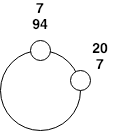
\includegraphics{math38}\\
Считаем по обеим дугам количество стульев, включая один из двух крайних: $20 - 7 + 94 - 7 = 100$.
Ответ: 100.

\subsection*{Задача 3.9}
Пусть $a, b, c, d, e$ -- количество шаров в 1, 2, 3, 4 и 5 часы соответственно.
$a\geq b\geq c\geq d\geq e$, $a+b+c+d+e=100$, $b+d<=a+c$, требуется найти $\min{(a + c + e)}$. Данная задача сводится к поиску $\max{(b + d)}$. Так как $b+d<=a+c$, а $a+b+c+d+e=100$, то $b+d\leq 100/2 = 50$. Такой случай легко придумать: $a, b, c, d, e = 25, 25, 25, 25, 0$. Таким образом, $\min{(a + c + e)} = 100 - \max{(b + d)} = 50$.
Ответ: 50.

\subsection*{Задача 3.10}
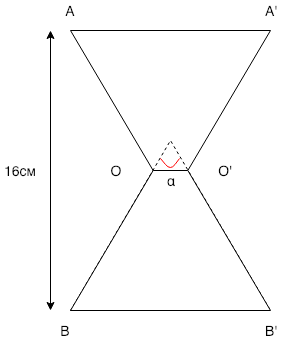
\includegraphics{math310}\\
Рассмотрим один из конусов.\\
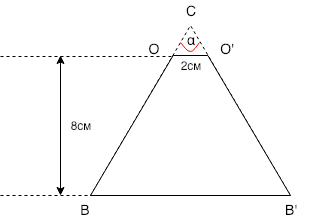
\includegraphics{math310_2}\\
$$\tg^2\alpha + 1 = \frac{1}{cos^2\alpha},$$
$$cos\alpha = \frac{3}{5}.$$ 
Пусть $OC = O'C = x$, по теореме косинусов: 
$OO'^2 = x^2 + x^2 - 2x\cdot x\cos\alpha = \frac{4x^2}{5},$
$x = \sqrt{5}.$
Опустим перпендикуляр $CO''$ к $OO''$. 
$$CO'' = \sqrt{x^2 - {OO''^2}} = \sqrt{5 - 1} = 2$$ 
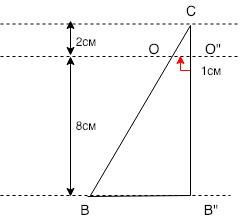
\includegraphics{math310_3}\\
Из подобия треугольников $BB'' = 5$. Объем песочных часов, т.е. удвоенный объем усеченного конуса, равен $$V=\frac{2}{3}\pi O''B''(OO''^2 + OO''BB'' + BB''^2)=\frac{2\pi}{3}\cdot 8 \cdot(1 + 5 + 25) = 519.409 \approx 519.$$
Ответ: 519.


\end{document}